\chapter{Testowanie rozwiązania}
\section{Środowisko testowe}
Wszystkie rozwiązania testowane będą przy użyciu następującego środowiska testowego:
\begin{description}
\item{Maszyna fizyczna:}
    \begin{itemize}
	\item CPU: \texttt{Intel(R) Core(TM)2 Quad CPU    Q9400 @ 2.66GHz} posiadający wsparcie dla wirtualizacji (\textit{VT-x})
	\item Pamięć RAM: \texttt{8G DDR2}
%%	\item OS: \texttt{Linux redraptor 3.18.1-gentoo \#7 SMP Wed Dec 31 02:04:37 CET 2014 x86\_64}
	\item OS: \texttt{Gentoo Linux 64bit, kernel 3.18.1}
	\item Platforma wirtualizacyjna: \texttt{KVM} (host)
    \end{itemize}
\item{Maszyna wirtualna na potrzeby kontenerów:}
    \begin{itemize}
	\item CPU: Mapowany z maszyny fizycznej. Przydział 3 rdzeni
	\item Pamięć RAM: \texttt{2G}
%%	\item OS: \texttt{Linux lxc 3.13.0-24-generic \#46-Ubuntu SMP Thu Apr 10 19:11:08 UTC 2014 x86\_64 x86\_64 x86\_64}
	\item OS: \texttt{Ubuntu Linux 64 bit, kernel 3.13.0-24-generic}
	\item Platforma wirtualizacyjna: \texttt{KVM} (guest), \texttt{LXC} (host)
    \end{itemize}
\item{Kontenery \texttt{LXC} do celów testowania aplikacji:}
    \begin{itemize}
	\item OS: Ubuntu linux. Jądra współdzielone z maszyną hostującą.
	\item Ustawienia \texttt{cgroups}: \texttt{lxc.cgroup.cpu.cfs\_quota\_us = 30000}
    \end{itemize}
\item{Maszyna wirtualna na potrzeby \texttt{LVS}:}
    \begin{itemize}
	\item CPU: Mapowany z maszyny fizycznej. Przydział 1 rdzeń
%%    	\item OS: \texttt{Linux mgr10 3.13.0-24-generic \#46-Ubuntu SMP Thu Apr 10 19:11:08 UTC 2014 x86\_64 x86\_64 x86\_64}
	\item OS: \texttt{Ubuntu Linux 64 bit, kernel 3.13.0-24-generic}
	\item Pamięć RAM: \texttt{192M}
    \end{itemize}
\end{description}
Aplikacje działające w \texttt{userspace}, tj. \texttt{apache, nginx, haproxy, php-fpm}, zostają uruchamiane w dedykowanych kontenerach \texttt{LXC}.
Usługi działające w warstwie jądra, tj. \texttt{LVS} zostają uruchomione na dedykowanej maszynie wirtualnej przy użyciu \texttt{KVM}.
\section{Wybór serwera WWW}
\label{sec:wybor}
W rozdziale tym zostanie przedstawione zestawienie kilku testów wydajnościowych dwóch serwerów WWW\@.
\begin{itemize}
\item Apache2
\item Nginx
\end{itemize}
Przetestowane zostanie serwrowanie plików statycznych oraz treści dynamicznych PHP{.}\\
Wszystkie testy zostały przeprowadzone z wykorzystaniem 10 000 połączeń.\\
Wszystkie czasy zostały podane w milisekundach.
\subsection{Pliki statyczne}
Testy plików statycznych przeprowadzone zostaną przy użyciu dwóch plików HTML{.}
Jeden o rozmiarze 10 bajtów, drugi o rozmiarze 100 kilobajtów.

\begin{figure}
	\centering
	\begin{subfigure}[h]{0.3\textwidth}
		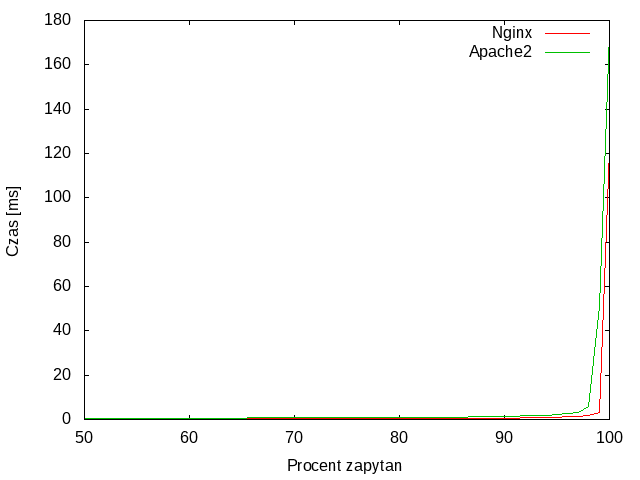
\includegraphics[width=\textwidth]{testy/wybor_index_maly_1.png}
		\caption{1 równoległe zapytanie}
	\end{subfigure}
	\begin{subfigure}[h]{0.3\textwidth}
		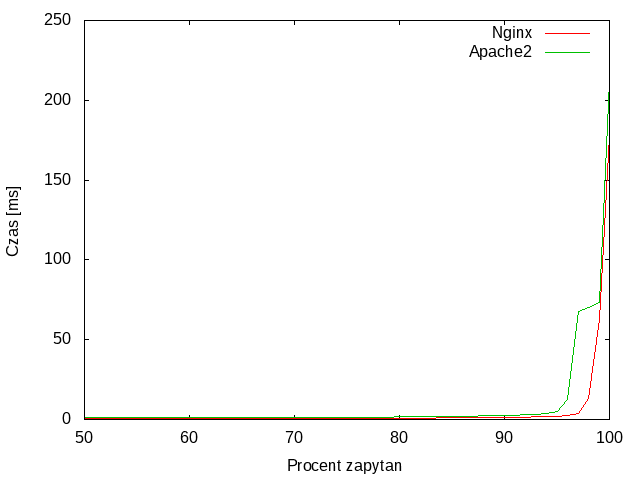
\includegraphics[width=\textwidth]{testy/wybor_index_maly_2.png}
		\caption{2 równoległe zapytania}
	\end{subfigure}
	\begin{subfigure}[h]{0.3\textwidth}
		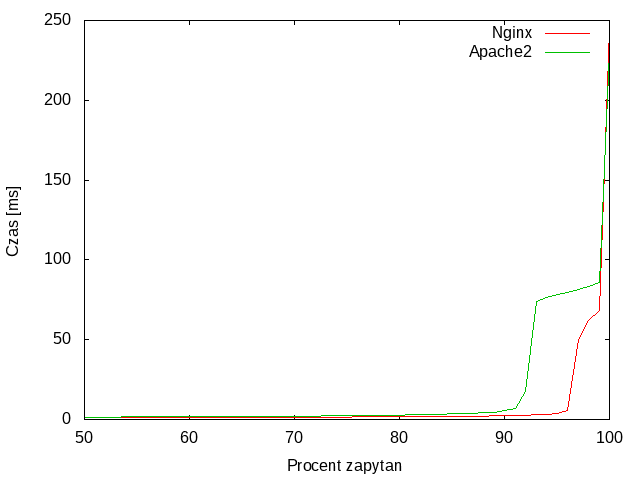
\includegraphics[width=\textwidth]{testy/wybor_index_maly_4.png}
		\caption{4 równoległe zapytania}
	\end{subfigure}

	\begin{subfigure}[h]{0.3\textwidth}
		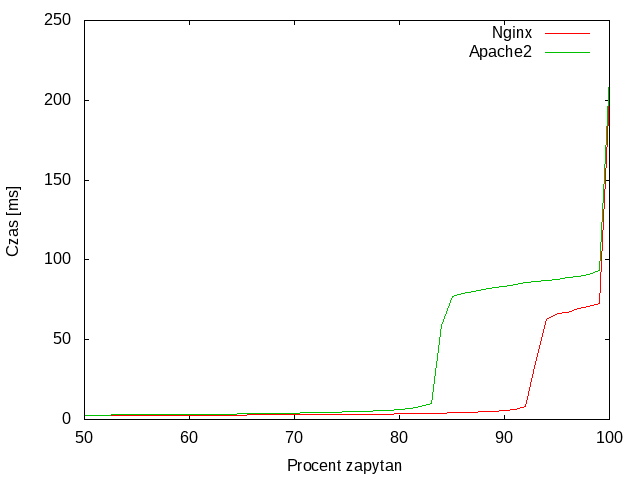
\includegraphics[width=\textwidth]{testy/wybor_index_maly_8.png}
		\caption{8 równoległych zapytań}
	\end{subfigure}
	\begin{subfigure}[h]{0.3\textwidth}
		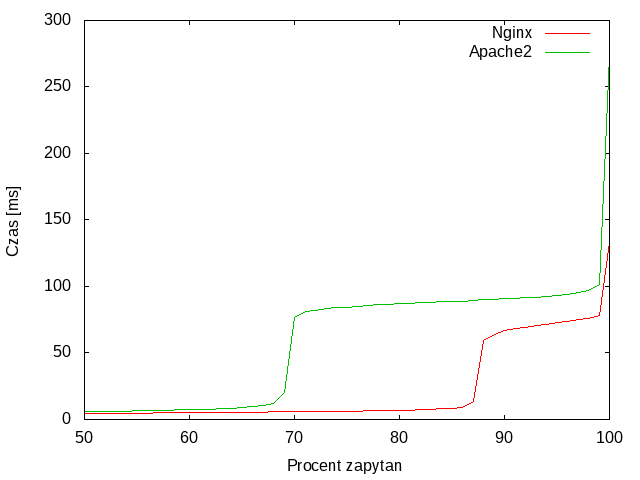
\includegraphics[width=\textwidth]{testy/wybor_index_maly_16.png}
		\caption{16 równoległych zapytań}
	\end{subfigure}
	\begin{subfigure}[h]{0.3\textwidth}
		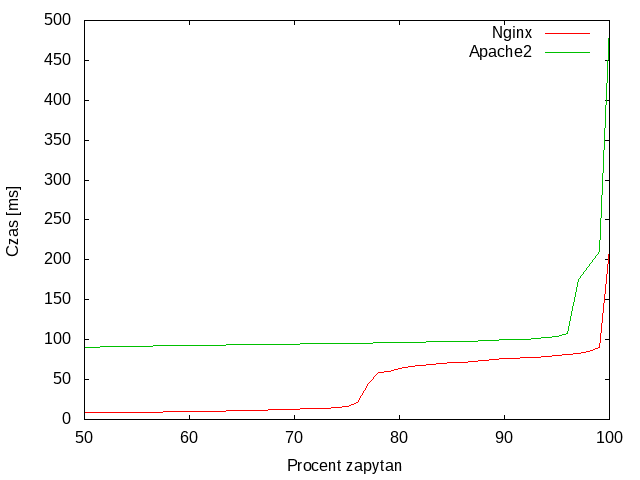
\includegraphics[width=\textwidth]{testy/wybor_index_maly_32.png}
		\caption{32 równoległe zapytania}
	\end{subfigure}

	\begin{subfigure}[h]{0.3\textwidth}
		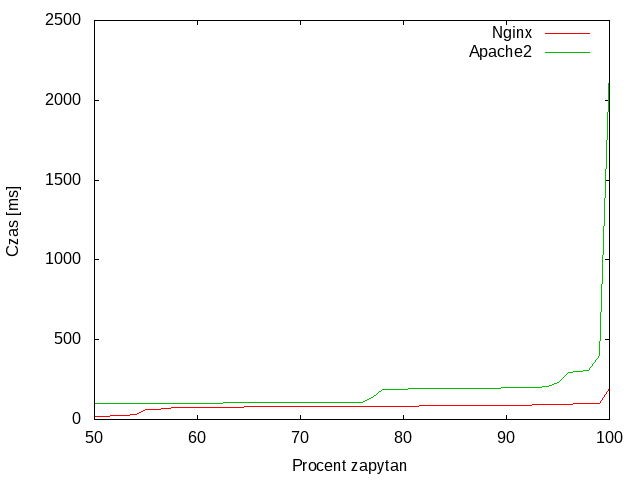
\includegraphics[width=\textwidth]{testy/wybor_index_maly_64.png}
		\caption{64 równoległe zapytania}
	\end{subfigure}
	\begin{subfigure}[h]{0.3\textwidth}
		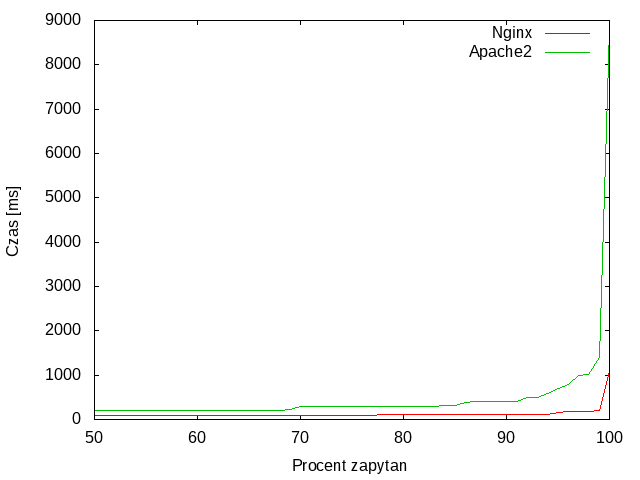
\includegraphics[width=\textwidth]{testy/wybor_index_maly_128.png}
		\caption{128 równoległe zapytania}
	\end{subfigure}
	\begin{subfigure}[h]{0.3\textwidth}
		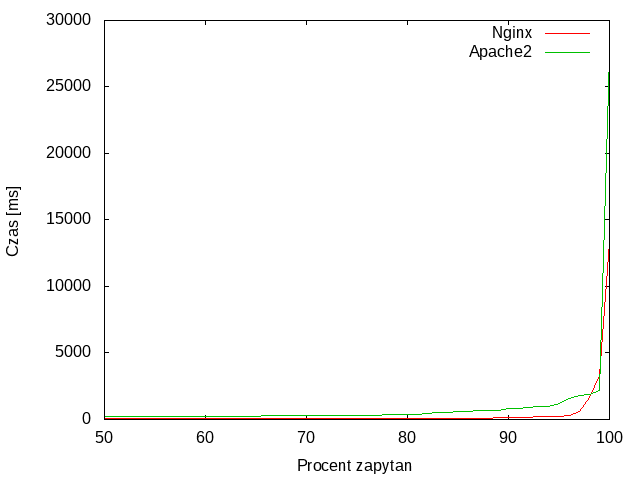
\includegraphics[width=\textwidth]{testy/wybor_index_maly_256.png}
		\caption{256 równoległych zapytań}
	\end{subfigure}
	\caption{Zapytania o mały plik statyczny}\label{fig:wyb_index_maly}
\end{figure}
\begin{figure}
	\centering
	\begin{subfigure}[h]{0.3\textwidth}
		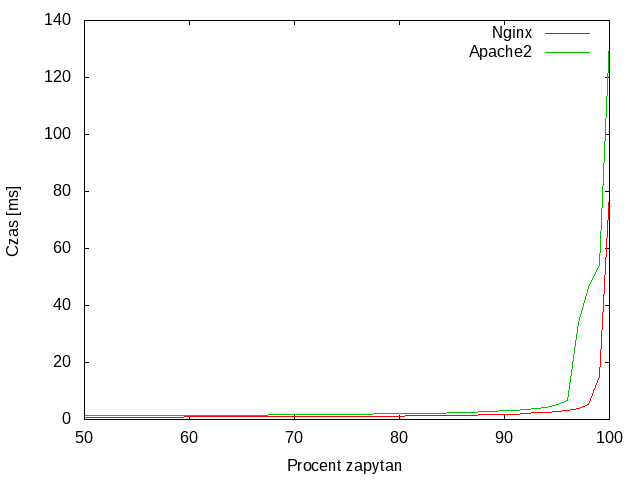
\includegraphics[width=\textwidth]{testy/wybor_index_duzy_1.png}
		\caption{1 równoległe zapytanie}
	\end{subfigure}
	\begin{subfigure}[h]{0.3\textwidth}
		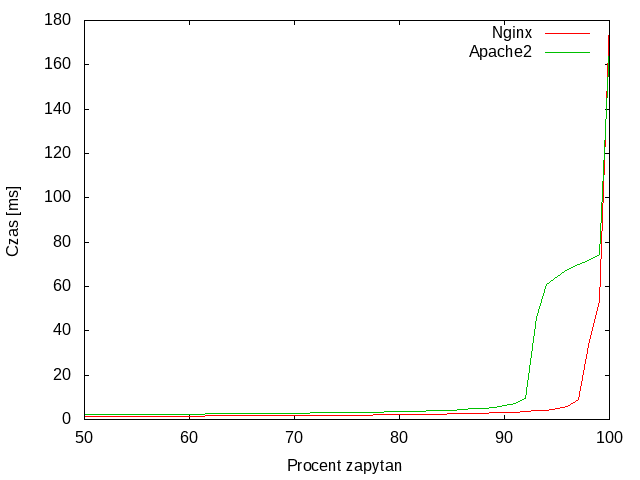
\includegraphics[width=\textwidth]{testy/wybor_index_duzy_2.png}
		\caption{2 równoległe zapytania}
	\end{subfigure}
	\begin{subfigure}[h]{0.3\textwidth}
		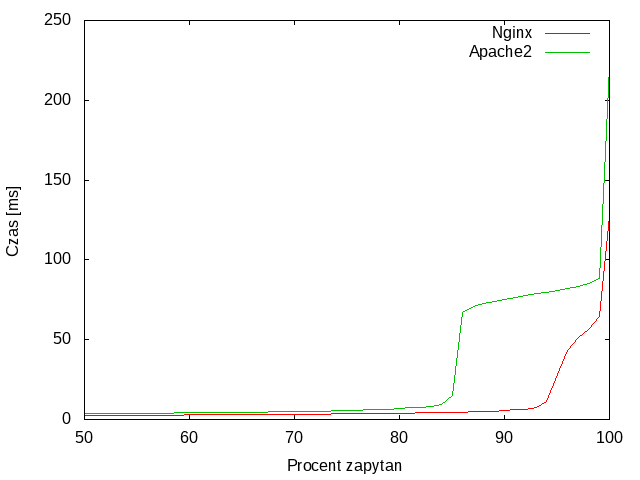
\includegraphics[width=\textwidth]{testy/wybor_index_duzy_4.png}
		\caption{4 równoległe zapytania}
	\end{subfigure}

	\begin{subfigure}[h]{0.3\textwidth}
		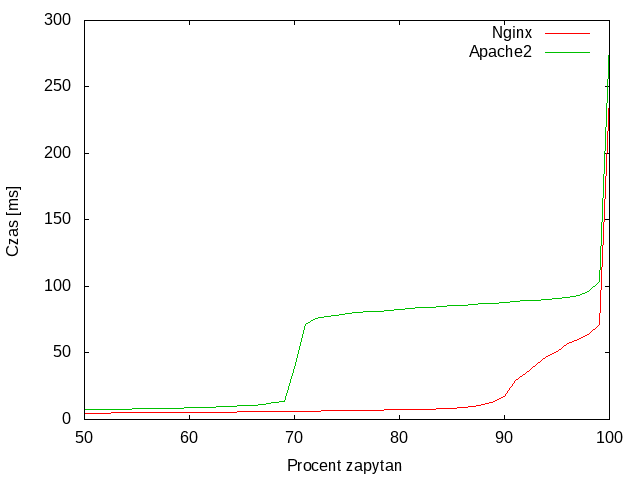
\includegraphics[width=\textwidth]{testy/wybor_index_duzy_8.png}
		\caption{8 równoległych zapytań}
	\end{subfigure}
	\begin{subfigure}[h]{0.3\textwidth}
		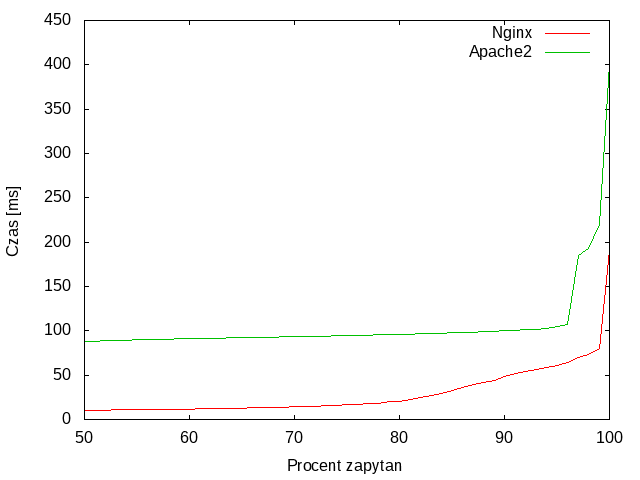
\includegraphics[width=\textwidth]{testy/wybor_index_duzy_16.png}
		\caption{16 równoległych zapytań}
	\end{subfigure}
	\begin{subfigure}[h]{0.3\textwidth}
		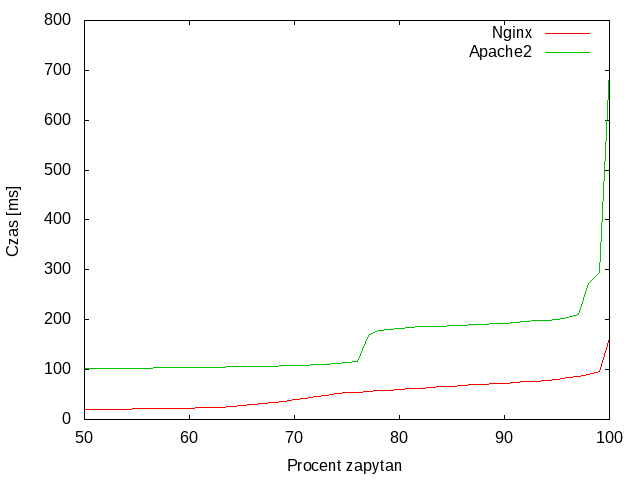
\includegraphics[width=\textwidth]{testy/wybor_index_duzy_32.png}
		\caption{32 równoległe zapytania}
	\end{subfigure}

	\begin{subfigure}[h]{0.3\textwidth}
		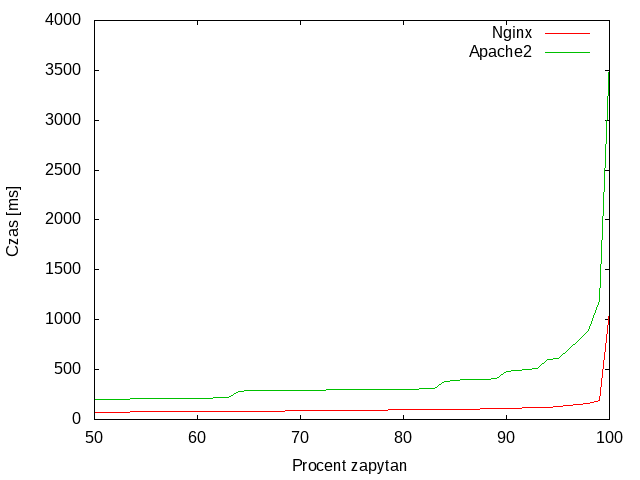
\includegraphics[width=\textwidth]{testy/wybor_index_duzy_64.png}
		\caption{64 równoległe zapytania}
	\end{subfigure}
	\begin{subfigure}[h]{0.3\textwidth}
		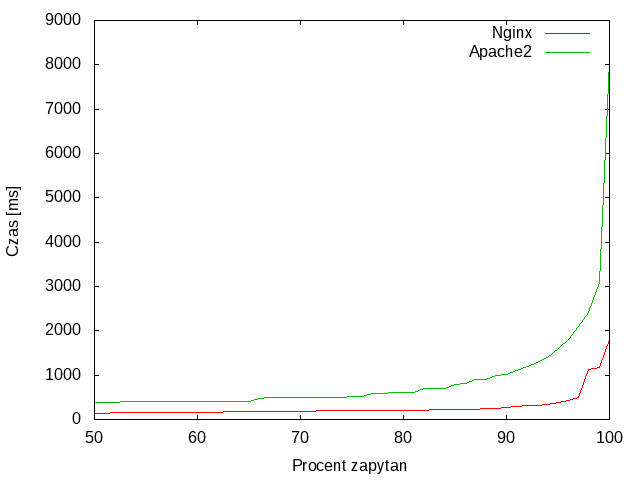
\includegraphics[width=\textwidth]{testy/wybor_index_duzy_128.png}
		\caption{128 równoległe zapytania}
	\end{subfigure}
	\begin{subfigure}[h]{0.3\textwidth}
		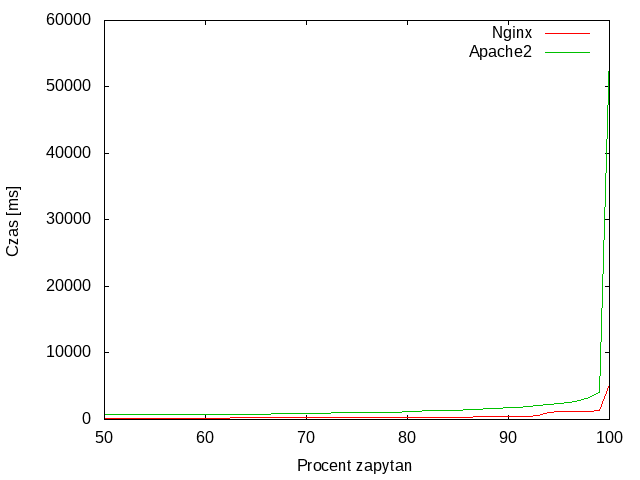
\includegraphics[width=\textwidth]{testy/wybor_index_duzy_256.png}
		\caption{256 równoległych zapytań}
	\end{subfigure}
	\caption{Zapytania o duży plik statyczny}\label{fig:wyb_index_duzy}
\end{figure}
Wykresy na rys.~\ref{fig:wyb_index_maly} przedstawiają czasy obsłużenia zapytań o plik HTML o rozmiarze 10 bajtów, natomiast wykresy na rys.~\ref{fig:wyb_index_duzy} czasy zapytań o plik o rozmiarze 100 kilobajtów.\\
Można zauważyć, że wyniki dla małych plików statycznych są zbliżone zarówno dla Apache jak i Nginx z lekką przewagą dla Nginx.
Największą przewagę Nginx-a widać przy średnim i dużym obciążeniu.
\clearpage
\subsection{Treść dynamiczna}
Testy treści dynamicznej przeprowadzane są przy użyciu konfiguracji Nginx + php-fpm oraz Apache + php-fpm.
Konfiguracja Apache + mod\_php została odrzucona, ponieważ wymaga umieszczenia serwera WWW oraz serwera PHP na jednym serwerze, co uniemożliwia użycie wielu serwerów PHP dla jednego serwera WWW.\\
Do testów zostały wykorzystane dwa bliźniacze skrypty obliczające liczby ciągu Fibonacciego.
Jeden ze skryptów został przedstawiony na listingu~\ref{lst:fib}.
Obliczane są wyrazy: piąty --- dla skryptu wykonującego się szybko, oraz piętnasty --- dla skryptu wykonującego się dłużej.\\
Wykorzystany został model obliczanie wartości rekurencyjny, ponieważ w przeciwieństwie do iteracyjnego wymaga większej mocy obliczeniowej.
Jest to pożądane aby czas obsługi zapytania obejmował czas wykonywania skryptu, a nie jedynie obsługi sesji HTTP oraz transferu danych (zostało to przetestowane przy wykorzystaniu \textit{szybkiego skryptu}).
\lstinputlisting[caption=fib.php,label=lst:fib,language=php]{lst/fib.php}
\begin{figure}
	\centering
	\begin{subfigure}[h]{0.3\textwidth}
		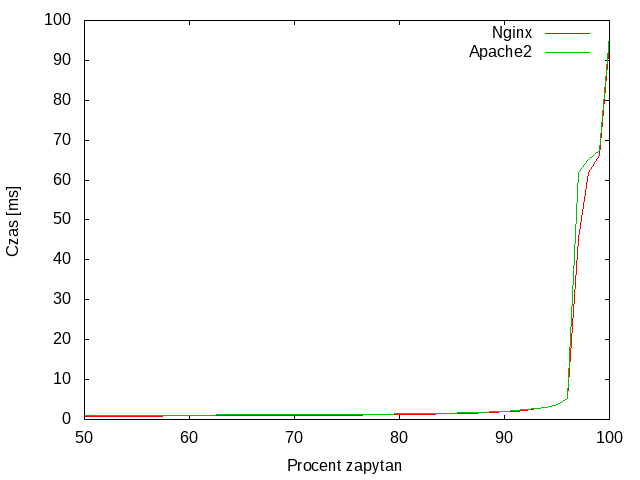
\includegraphics[width=\textwidth]{testy/wybor_fib_5_1.png}
		\caption{1 równoległe zapytanie}
	\end{subfigure}
	\begin{subfigure}[h]{0.3\textwidth}
		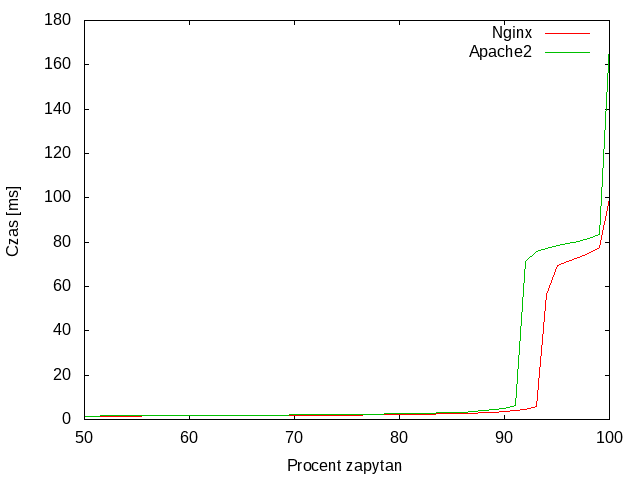
\includegraphics[width=\textwidth]{testy/wybor_fib_5_2.png}
		\caption{2 równoległe zapytania}
	\end{subfigure}
	\begin{subfigure}[h]{0.3\textwidth}
		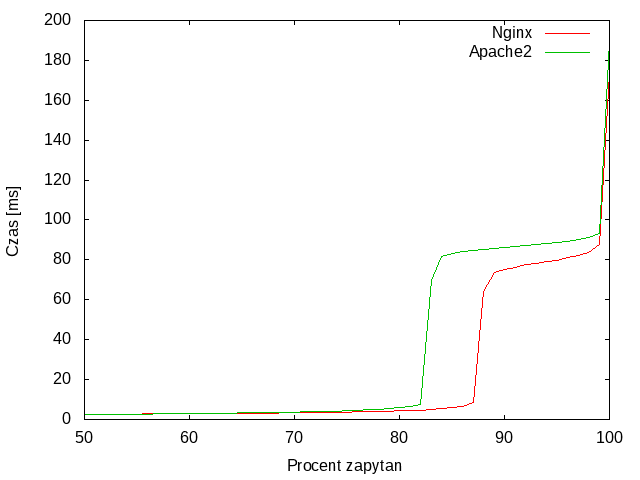
\includegraphics[width=\textwidth]{testy/wybor_fib_5_4.png}
		\caption{4 równoległe zapytania}
	\end{subfigure}

	\begin{subfigure}[h]{0.3\textwidth}
		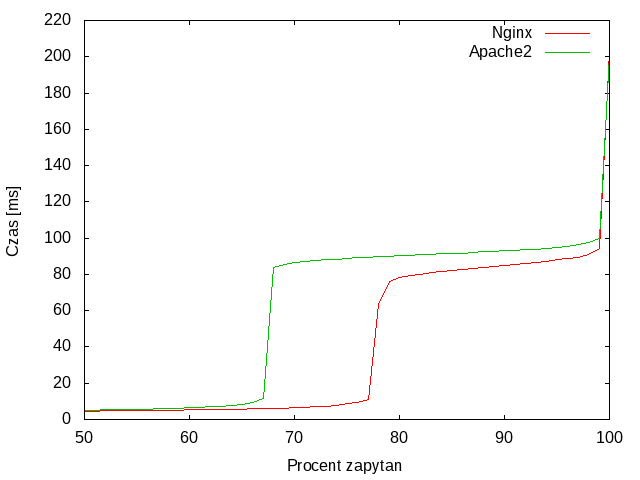
\includegraphics[width=\textwidth]{testy/wybor_fib_5_8.png}
		\caption{8 równoległych zapytań}
	\end{subfigure}
	\begin{subfigure}[h]{0.3\textwidth}
		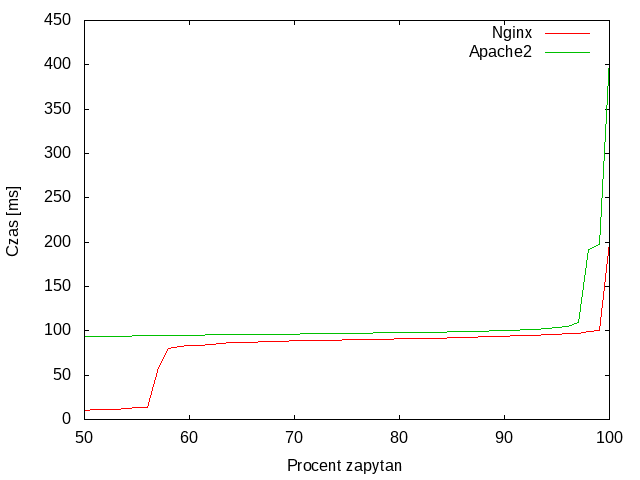
\includegraphics[width=\textwidth]{testy/wybor_fib_5_16.png}
		\caption{16 równoległych zapytań}
	\end{subfigure}
	\begin{subfigure}[h]{0.3\textwidth}
		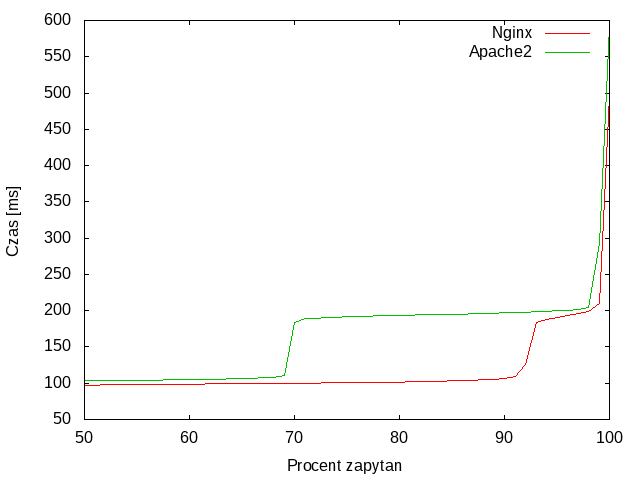
\includegraphics[width=\textwidth]{testy/wybor_fib_5_32.png}
		\caption{32 równoległe zapytania}
	\end{subfigure}

	\begin{subfigure}[h]{0.3\textwidth}
		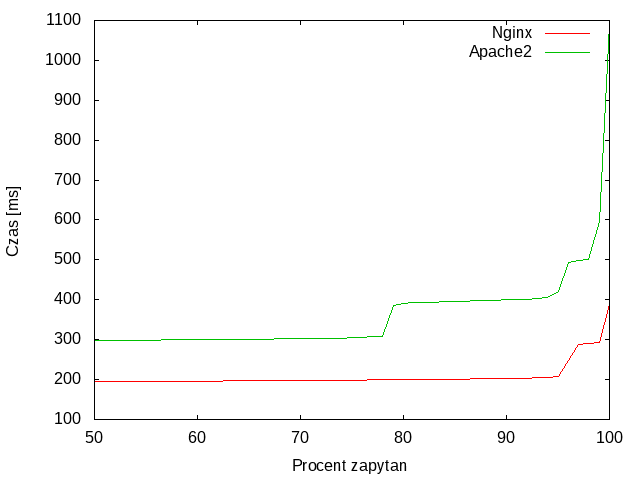
\includegraphics[width=\textwidth]{testy/wybor_fib_5_64.png}
		\caption{64 równoległe zapytania}
	\end{subfigure}
	\begin{subfigure}[h]{0.3\textwidth}
		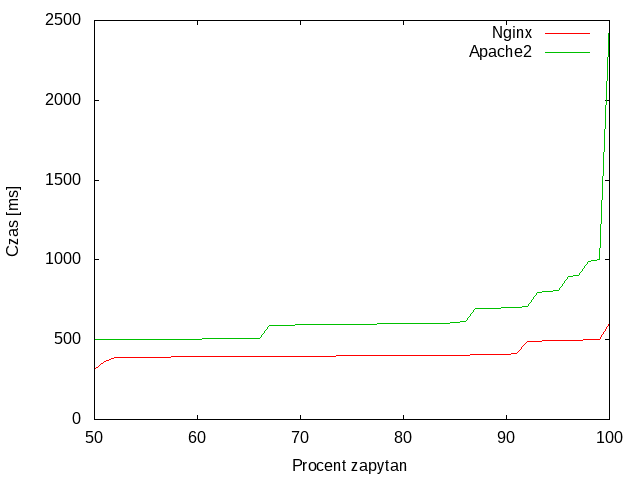
\includegraphics[width=\textwidth]{testy/wybor_fib_5_128.png}
		\caption{128 równoległe zapytania}
	\end{subfigure}
	\begin{subfigure}[h]{0.3\textwidth}
		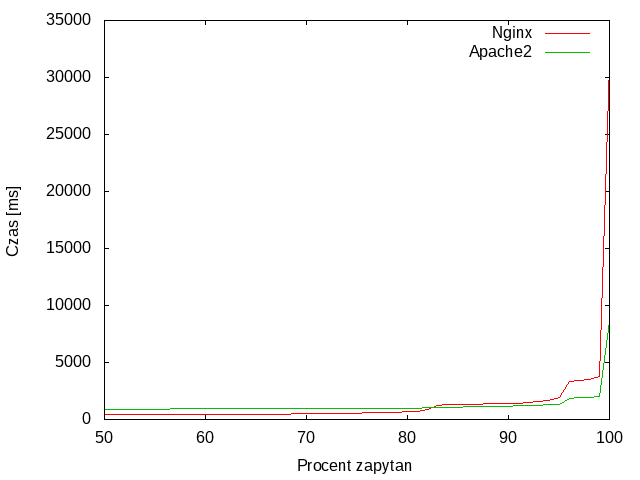
\includegraphics[width=\textwidth]{testy/wybor_fib_5_256.png}
		\caption{256 równoległych zapytań}
	\end{subfigure}
	\caption{Zapytania o szybki skrypt PHP}\label{fig:wyb_fib_5}
\end{figure}
\begin{figure}
	\centering
	\begin{subfigure}[h]{0.3\textwidth}
		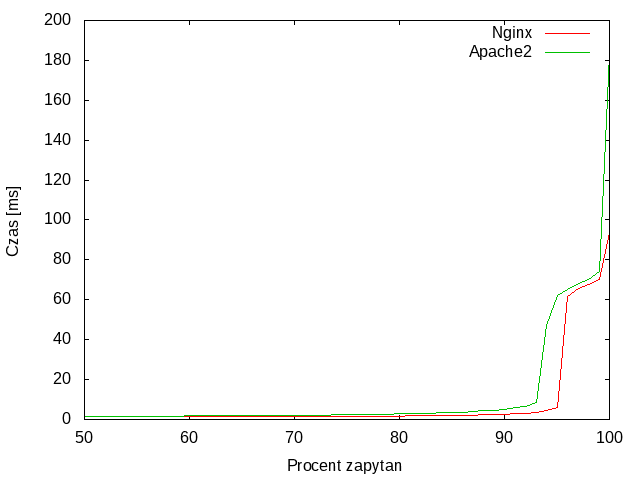
\includegraphics[width=\textwidth]{testy/wybor_fib_15_1.png}
		\caption{1 równoległe zapytanie}
	\end{subfigure}
	\begin{subfigure}[h]{0.3\textwidth}
		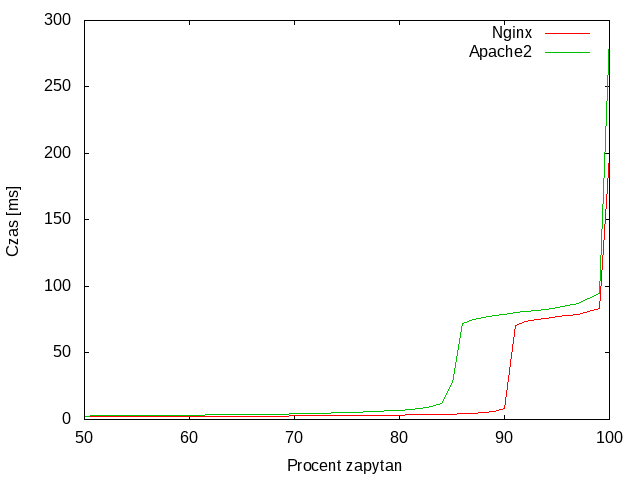
\includegraphics[width=\textwidth]{testy/wybor_fib_15_2.png}
		\caption{2 równoległe zapytania}
	\end{subfigure}
	\begin{subfigure}[h]{0.3\textwidth}
		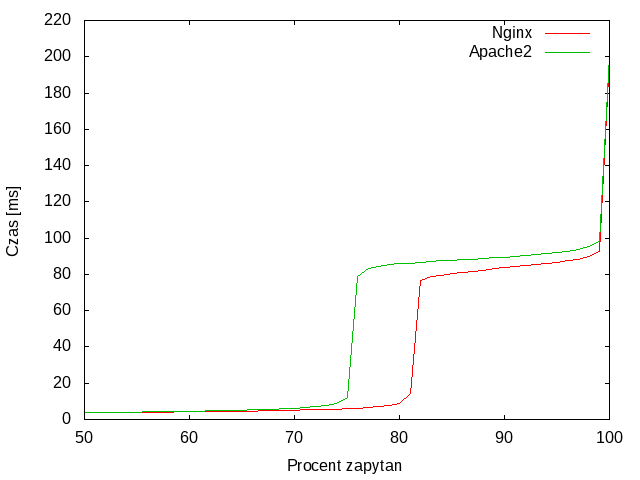
\includegraphics[width=\textwidth]{testy/wybor_fib_15_4.png}
		\caption{4 równoległe zapytania}
	\end{subfigure}

	\begin{subfigure}[h]{0.3\textwidth}
		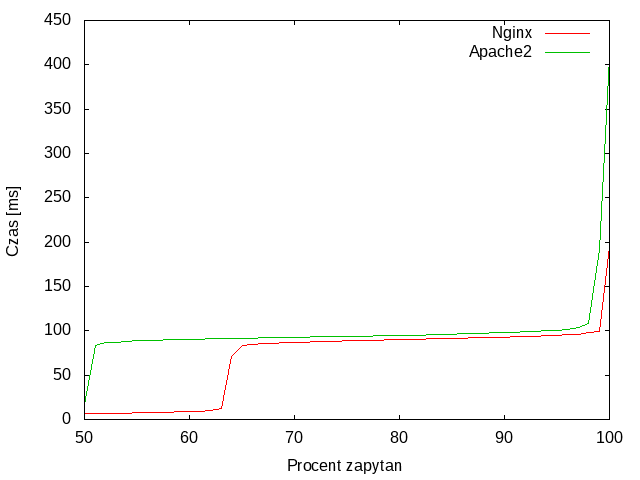
\includegraphics[width=\textwidth]{testy/wybor_fib_15_8.png}
		\caption{8 równoległych zapytań}
	\end{subfigure}
	\begin{subfigure}[h]{0.3\textwidth}
		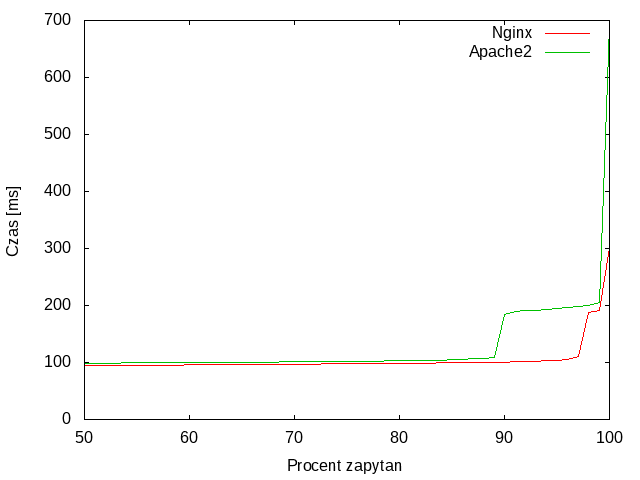
\includegraphics[width=\textwidth]{testy/wybor_fib_15_16.png}
		\caption{16 równoległych zapytań}
	\end{subfigure}
	\begin{subfigure}[h]{0.3\textwidth}
		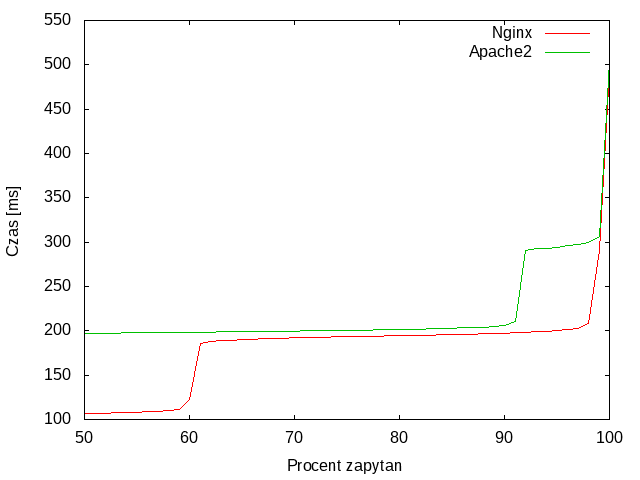
\includegraphics[width=\textwidth]{testy/wybor_fib_15_32.png}
		\caption{32 równoległe zapytania}
	\end{subfigure}

	\begin{subfigure}[h]{0.3\textwidth}
		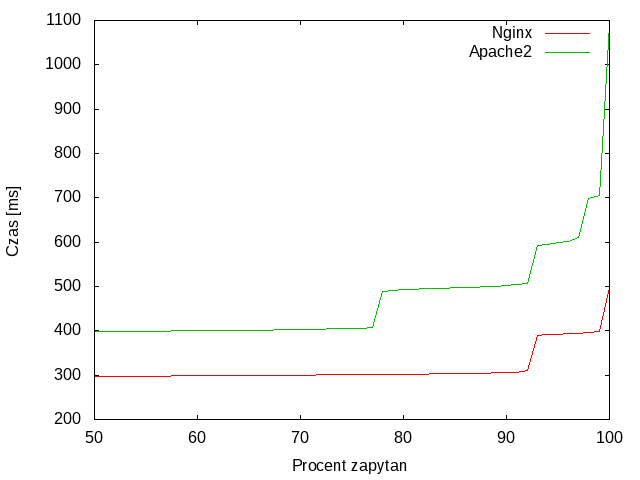
\includegraphics[width=\textwidth]{testy/wybor_fib_15_64.png}
		\caption{64 równoległe zapytania}
	\end{subfigure}
	\begin{subfigure}[h]{0.3\textwidth}
		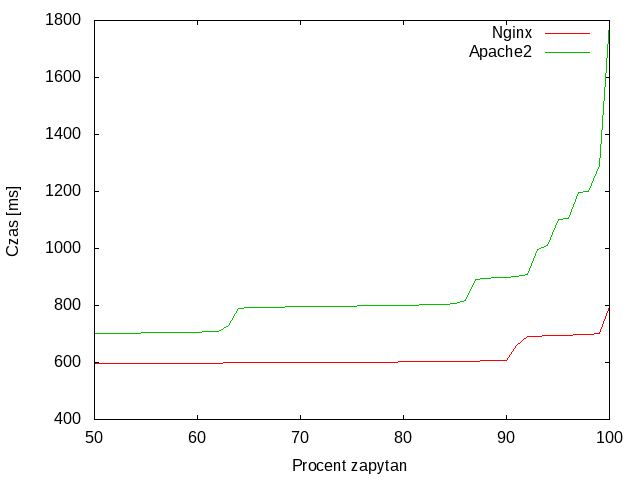
\includegraphics[width=\textwidth]{testy/wybor_fib_15_128.png}
		\caption{128 równoległe zapytania}
	\end{subfigure}
	\begin{subfigure}[h]{0.3\textwidth}
		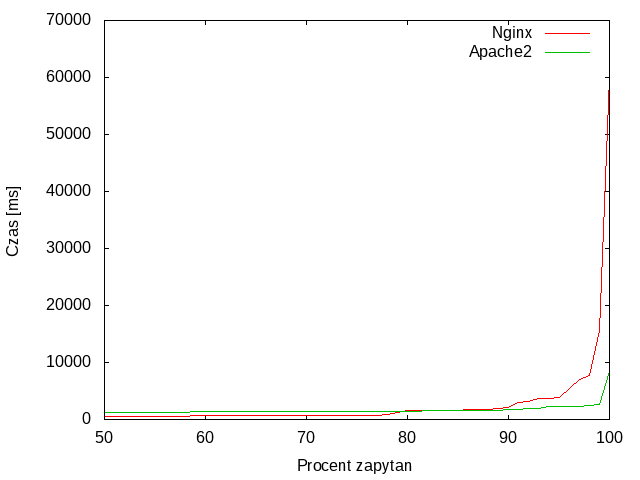
\includegraphics[width=\textwidth]{testy/wybor_fib_15_256.png}
		\caption{256 równoległych zapytań}
	\end{subfigure}
	\caption{Zapytania o wolny skrypt PHP}\label{fig:wyb_fib_15}
\end{figure}
Na wykresach~\ref{fig:wyb_fib_5} oraz~\ref{fig:wyb_fib_15} obrazujących czasy obsługi zapytań do skryptów PHP, można zauważyć że różnice pomiędzy Apache a Nginx są mniejsze niż dla plików statycznych.
Wynika to z faktu, ze obsługą zapytań w obu przypadkach zajmuje się PHP-fpm, natomiast serwer WWW odpowiedzialny jest jedynie za przekazywanie zapytań do \textit{backendu}.
\subsection{Podsumowanie}
Jak wykazały testy, Nginx daje krótsze czasy odpowiedzi we wszystkich testowanych sytuacjach, dlatego został wybrany jako podstawowy serwer wykorzystywany w przedstawionym projekcie.
\clearpage
\section{DNS round robin}
\subsection{Uwagi wstępne}
Jak zostało wspomniane w rozdziale~\ref{sec:dns}, DNS round robin nie jest metodą \textit{load balancingu} a jedynie wstępną metodą dystrybucji ruchu.
Pociąga to za sobą pewne konsekwencje.
Przeciętna aplikacja sieciowa, np: Chrome bądź links, dokonuje rozwiązania nazwy przy pierwszym odwołaniu się do danego adresu a następnie w celu zwiększenia wydajności, \textit{cachuje} jej adres.
Efektem tego takiego zachowania jest nawiązywanie późniejszych połączeń do tego samego adresu IP\@.
Aplikacja \textit{Apache Benchmark} która jest wykorzystywana do testowania rozwiązań w poniższej pracy również dokonywała jednorazowego rozwiązania nazwy i łączenia się do jednego adresu, co uniemożliwiało przeprowadzenie testów wydajnościowych \textit{DNS round robin} przy użyciu tego narzędzia.
Została zgłoszona poprawka\cite{ab_dnsrr} poprawiająca tą niedogodność.
Testy z wykorzystaniem tej poprawki symulują łączenie się dużej liczby niezależnych użytkowników.

Przy testowanie \textit{DNS round robin} nie zostanie przeprowadzona tak dokładna analiza jak przy wyborze serwera WWW, ponieważ metoda ta nie wpływa na działanie serwera WWW a jedynie na dystrybucję ruchu.

W testach tych, w przeciwieństwie do wyboru serwera WWW, użyto opcji \texttt{Keep Alive} powodującej utrzymywanie połączenia i wykonywanie kolejnych bez ponownego nawiązywania połączeń TCP\@.
W przypadku użycia poprawki~\cite{ab_dnsrr} każde połączenie jest tworzone do serwera wynikającego z technologi \textit{DNS round robin} a następnie jest ono utrzymywane aż do zakończenia programu. Liczba połączeń zależy od parametru \texttt{concurrent}
\subsection{Testy wydajnościowe}
Testowanie rozwiązania \textit{DNS round robin} zostanie przedstawione na odpytywaniu jedynie pliku statycznego ponieważ testy dla pozostałych treści będą analogiczne do tych przedstawionych w rozdziale~\ref{sec:wybor}.\\
Do testów został wykorzystany \textit{DNS round robin} przedstawiony na listingu~\ref{lst:test_dnsrr}.
\lstinputlisting[caption=DNS round robin, label=lst:test_dnsrr]{lst/test_dnsrr.bash}
Zawiera on cztery serwery z identyczną konfiguracją.\\
Wykresy~\ref{fig:test_dnsrr} przedstawiają czasy obsługi zapytań w przypadku pojedynczego serwera WWW oraz grupy serwerów z dystrybucją ruchu poprzez \textit{DNS round robin}.
Na wykresach został pominięty czas najdłuższego połączenia z powodu małego wkładu informacyjnego oraz dużego stopnia zaciemniania obrazu.
\wykresy{dnsrr}{Dystrybuja ruchu w oparciu o DNS RR}{test_dnsrr}
Tabela~\ref{tab:test_dnsrr} przedstawia liczbę obsłużonych zapytań na sekundę.
\begin{table}[h]
\centering
\begin{tabular}{cccc}
	\toprule
	Liczba połączeń & Nginx & DNS RR & Przyrost\\
	\midrule
	\midrule
	1&2571&4301& +67\%\\
	\midrule
	2&2001&5458& +172\%\\
	\midrule
	4&1353&6264& +362\%\\
	\midrule
	8&1704&7582& +344\%\\
	\midrule
	16&2097&8720& +315\%\\
	\midrule
	32&2133&7484& +250\%\\
	\midrule
	64&1968&10617& +439\%\\
	\midrule
	128&1945&10194& +424\%\\
	\midrule
	256&2190&9821& +348\%\\
	\bottomrule
\end{tabular}
\caption{Obsłużonych zapytań na sekundę}
\label{tab:test_dnsrr}
\end{table}
\subsection{Podsumowanie}
Jak można zaobserwować na wykresach, użycie dystrybucji ruchy zmniejsza czasy oczekiwania na przetworzenie zapytań.\\
Dane przedstawione w tabeli~\ref{tab:test_dnsrr} pokazują, iż użycie czterech serwerów zamiast jednego daje w większości przypadków przyrost ok 300\%, co jest wartością oczekiwaną, ponieważ przy użyciu trzech dodatkowych serwerów oczekujemy trzykrotnego przyrostu wydajności.\\
W przypadku jednego równoległego połączenia oczekiwanym przyrostem były przyrost 0\% ponieważ wykonywane jest jedno połączenie, jednak specyfika serwera Nginx jest taka, że po przyjęciu stu połączeń w trybie \texttt{Keep-Alive} zamyka on połączenie.
Następuje wtedy nawiązanie kolejnego, które zostaje przekierowane do kolejnego serwera z puli \textit{DNS round robin}.
Jest to przyczyną zwiększonego przyrostu dla jednego i dwóch równoległych połączeń.\\
Przy liczbie połączeń cztery i więcej powyższy efekt nie ma znaczenia, ponieważ w obsłudze zapytań biorą udział wszystkie serwery.
\section{LVS}
W tej sekcji przetestowany zostanie LVS w trybie \textit{direct routing}, ponieważ jest on najrozsądniejszym trybem.
Testom poddany zostanie narzut wynikający z użycia LVS, jak również przetestowane zostaną rozwiązanie bliższe rzeczywistości, czyli zawierające kilka \textit{real server}-ów.
Ponadto, sprawdzone zostanie zachowanie LVS w warunkach nieidealnych, tj.\ w przypadku awarii jednego z \textit{real server}-ów oraz w przypadku wysycenia łącza.
\subsection{Uwagi dotyczące urządzeń sieciowych}
\label{sub:uwagi_sieciowe}
Ponieważ w omawianym rozwiązaniu występuje jeden węzeł do którego nawiązywane są połączenia, parametry łącza są w tym przypadku (w przeciwieństwie do DNS round robin gdzie klient łączy się do różnych serwerów) istotne.
\begin{description}
	\item{Maszyna z \textit{directorem}}
		\begin{itemize}
			\item Wirtualizowany sterownik karty sieciowej: rtl8139
			\item Szybkość karty podawana przez ethtool: 100Mb/s
		\end{itemize}
	\item{Maszyna z LXC}
		\begin{itemize}
			\item Wirtualizowany sterownik karty sieciowej: virtio
			\item Szybkość karty podawana przez ethtool: Brak
		\end{itemize}
	\item{Maszyna z Nginx}
		\begin{itemize}
			\item Wirtualizowany sterownik karty sieciowej: wirtualny interface hosta
			\item Szybkość karty podawana przez ethtool: 10000Mb/s
		\end{itemize}
\end{description}
Na uwagę zasługują tutaj parametry maszyny będącej hostem dla LXC\@.
Użycie sterownika \texttt{virtio} pozwala maszynie wirtualizowanej komunikować się z maszyną hostującą bez emulacji konkretnych sterowników sieciowych, lecz już na poziomie jądra.
Dlatego nie jest możliwe określenie prędkości takiego interface-u, ponieważ zasada jego działania jest inna niż rzeczywistych kart sieciowych.\\
Podobnie sytuacja wygląda dla kontenerów LXC\@.
Tam komunikacja następuje poprzez wirtualne interface-y na jeden maszynie, dlatego prędkość podana przez \texttt{ethtool} wynosi 10Gb/s.

W przypadku testowania zachowania rozwiązania na wysycenie łącza, prędkość interface-u na maszynie z \textit{directorem} zostanie ustawiona na 10Mb/s.
Pozwoli to zasymulować sytuacje w której żądany ruch będzie większy niż możliwości łącza serwera.
\subsection{Narzut własny LVS}
\label{sec:lvs_narzut}
Aby sprawdzić jakie opóźnienie generuje mechanizm LVS, skonfigurowany zostanie jeden serwer \textit{director} oraz jeden \textit{real server}.
Porównując czasy odpowiedzi serwera WWW odpytywanego bezpośrednio oraz poprzez LVS, otrzymamy jaki wpływ na działanie ma LVS\@.
Żądany będzie mały plik statyczny.
\wykresy{one_lvs_maly}{Narzut własny LVS}{one_lvs_maly}

Jak widać na rysunku~\ref{fig:one_lvs_maly}, czasy odpowiedzi serwera bezpośrednio oraz poprzez LVS nie odbiegają zbytnio od siebie.
Różnica na wykresie jest widoczna jedynie dla jednego konkurencyjnego zapytania, jednak wartość tych czasów (0.2ms i 0.4ms) są na tyle małe, ze ta różnica może zostać pominięta.
\subsection{Wiele real serverów}
Rozważmy teraz przypadek, w którym mamy cztery takie same serwery WWW\@.
Zostały skonfigurowane 3 usługi LVS\@. Tą konfiguracje przedstawia listing~\ref{lst:four_lvs_maly}.
\footnotesize
\lstinputlisting[caption=LVS z wieloma serwerami,label=lst:four_lvs_maly]{lst/four_lvs_maly}
\normalsize
Widzimy, ze każda z usług posiada inną liczę serwerów oraz posiada taki sam algorytm balansowania.
Każdy z serwerów ma wagę 1 oraz każdy jest wykorzystywany w trybie \textit{direct routing}.

\wykresy{four_lvs_maly}{Czasy odpowiedzi w zależności od ilości serverów}{four_lvs_maly}
Wykresy~\ref{fig:four_lvs_maly} przedstawiają czasy odpowiedzi w zależności o ilości \textit{real server}-ów.
Wymaga on trochę dokładniejszej analizy niż poprzednie wykresy.
Dla jednego równoległego zapytania, widzimy ze czasy każdej z usług LVS są gorsze niż bezpośrednie zapytania do server WWW\@.
Dzieje się tak dlatego, ze mając jedno równoczesne zapytanie, wykorzystywany jest tylko jeden serwer na raz, czyli jest to sytuacja tożsama z rozdziałem~\ref{sec:lvs_narzut}.\\
W przypadku 2 połączeń, wykresy zaczynają się zbiegać, ponieważ narzut LVS zaczyna być kompensowany poprzez dystrybucję zapytań.\\
Począwszy od czterech zapytań, zauważamy że połączenia kierowane do LVS są obsługiwane szybciej.
Najbardziej jest to widoczne przy dużym obciążeniu serwera, tj. 128 i 256 równoległych zapytań.
